%Jennifer Pan, August 2011

\documentclass[10pt,letter]{article}
	% basic article document class
	% use percent signs to make comments to yourself -- they will not show up.
\usepackage{enumerate}
\usepackage{amsmath}
\usepackage{amssymb}
	% packages that allow mathematical formatting

\usepackage{graphicx}
	% package that allows you to include graphics

\usepackage{setspace}
	% package that allows you to change spacing

\onehalfspacing
	% text become 1.5 spaced

\usepackage{fullpage}
	% package that specifies normal margins
	

\begin{document}
	% line of code telling latex that your document is beginning


\title{Homework 1 Solution}

\author{SABIC: Physics}

\date{Due January 21, 2016}
	% Note: when you omit this command, the current dateis automatically included
 
\maketitle 
	% tells latex to follow your header (e.g., title, author) commands.

\section*{Reading (Due April 1, 2015):}
Read Chapter 1.
\section*{Problem 1: practice with estimation}
\begin{enumerate}[(a)]
\item {\bf How many kernels of corn does it take to fill a 2 liter soda bottle?}
\hspace{2pt}
2 liters is $2000 {\rm cm}^3$, and a kernel of corn is about $(0.5{\rm cm})^3 = .1 {\rm cm}^3$. So that puts us with $2000/.1 \simeq 10000$ kernels.
\item {\bf How many liters of gasoline are used in the United States in one day?}
\hspace{2pt}
There are let's say $100$ million = $10^8$ cars in the USA. Each car need to fill their gas tank once every other week ($\simeq 20$ days), and a gas tank holds $\simeq 20$L of gasoline. That means that each driver uses $\simeq 1$L of gas a day, and with $100$ million cars, we'd expect about $100$ million liters of gasoline a day.

\end{enumerate}
\section*{Problem 2: conceptual}
\begin{enumerate}[(a)]
\item {\bf What physical phenomena could you use to define a time standard?}
\hspace{2pt}
There are a bunch of good answers. You can use the sunrise to define a day, which is a good answer. The current answer has to do with a vibrational mode of a cesium atom, whose frequency is measured very precisely. That's how atomic clocks work.
\item  {\bf Describe how you could measure the thickness of a sheet of paper with an ordinary ruler.}
\hspace{2pt}
Take a bunch of identical papers and stack them, then divide the answer by the number of papers in the stack.
\item {\bf Can you find two vectors with different lengths that have a vector sum of zero? What length restrictions are required for three vectors to have a vector sum of zero? Explain your reasoning.}
\hspace{2pt}
To the first part, no, you can't: you need two vectors of the same magnitude to sum to zero, and in addition they have to point in exactly opposite directions. We call one of the vectors $\vec{v}$, then the other vector we call $-\vec{v}$.
\item {\bf (i) Does it make sense to say that a vector is negative?}
No. Vectors have a magnitude (which is always positive), and a direction, which is an angle and therefore also always positive. 
\hspace{2pt}
{\bf (ii) Does it make sense to say that one vector is the negative of another? Does your answer here contradict what you said in part (i)?}
Sure--that means a vector with the same magnitude pointing in the opposite direction. That's not contradictory, since we're not saying either $\vec{v}$ or $-\vec{v}$ is negative, just that they're negatives {\textit of each other.}


\end{enumerate}
\section*{Problem 3: vector addition}
\begin{figure}[!ht]
  \centering
    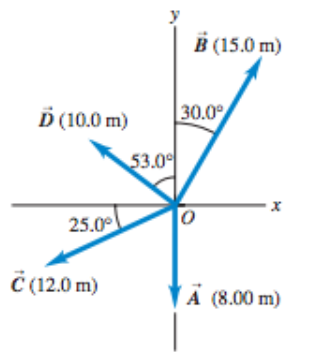
\includegraphics[width=0.5\textwidth]{fig1.png}
\end{figure}
\begin{enumerate}[(a)]
\item {\bf For the vectors $\vec{A}$ and $\vec{B} $in the figure, find the magnitude and direction of (i) $\vec{A} + \vec{B}$, (ii) $\vec{A} - \vec{B}$, (iii) $-\vec{A} - \vec{B}$, and (iv) $\vec{B} - \vec{A}$.}
\hspace{2pt}
To add vectors, you have to add components. I'll do out part (i) and then give the answers to the rest.
$\vec{A} = -8$m $\hat{j}$, and $\vec{B} = (15 \sin 30^\circ \hat{i} + 15 \cos 30^\circ \hat{j}$m $= 15/2 \hat{i} + 15\sqrt{3}/2 \hat{j}$. So $\vec{A} + \vec{B} = 15\sqrt{3}/2 \hat{i} - 0.5 \hat{j}$m. The magnitude is $|\vec{A} + \vec{B}| = \sqrt{(15/2)^2 + (15 \sqrt{3}/2 - 8)^2} = 9$, while the angle is $\tan^{-1}{V_y/V_x} = 34^\circ$ above the $x$-axis. For the others:
\begin{align}
|\vec{A} - \vec{B}| &= 22 {\rm m} :\, \, \simeq 70^\circ \text{ below the }-x \text{ axis.}\\
|-\vec{A} - \vec{B} | = |\vec{A} + \vec{B}| &= 9 :\,  \, \simeq 34^\circ \text{ below the }-x \text{ axis}\\
|\vec{B} - \vec{A}| = |\vec{A} - \vec{B}| &= 22 :\,  \, \simeq 70^\circ \text{ above the }x \text{ axis}
\end{align}
\item {\bf A spelunker is surveying a cave. She follows a passage 180 m straight west, then 210 m in a direction $45^\circ$ east of south, and then 280 m at $30^\circ$ east of north. After a fourth unmeasured displacement, she finds herself back where she started. Use a scale drawing to determine the magnitude and direction of the fourth displacement.}
Call the given vectos $\vec{A}$, $\vec{B}$, and $\vec{C}$, while the 4th displacement we want to find $\vec{D}$. Since she returns to where she started, we must have 
\begin{equation*}
\vec{A} + \vec{B} +\vec{C} + \vec{D} = 0
\end{equation*}
If you do the math (or draw really carefully), you find that the magnitude is $144$m, and the direction is $41^\circ$ South of West.
\end{enumerate}
\section*{Problem 4: vector multiplication}
\begin{enumerate}[(a)]
\item {\bf For the vectors $\vec{A}$, $\vec{B}$, and $\vec{C}$ in the figure, find $\vec{A}\cdot\vec{B}$, $\vec{A}\cdot\vec{C}$, and $\vec{B}\cdot\vec{C}$.}
$\vec{A}\cdot\vec{B}=|A||B|\cos (60^\circ - (-90^\circ)) = (8m)(15m)\cos 150^\circ = -104{\rm m}^2$. Similarly, we have $\vec{A} \cdot \vec{C} = 40.6 {\rm m}^2$, and $\vec{B}\cdot\vec{C} = -148 {\rm m}^2$. 
\item {\bf For the vectors $\vec{A}$ and $\vec{D}$ in the figure, find the magnitude and direction of $\vec{A} \times \vec{D}$ and $\vec{D} \times \vec{A}$.}
The magnitude of both is the same, and it's $|A||D|\sin 127^\circ = 63.9 {\rm m}^2$. By the right hand rule, $\vec{A} \times \vec{D}$ is in the $-z$ direction, while $\vec{D}\times\vec{A}$ is in the $+z$ direction.s
\end{enumerate}

\end{document}
	% line of code telling latex that your document is ending. If you leave this out, you'll get an error
